\documentclass[11pt,letterpaper]{article}
\usepackage[utf8]{inputenc}
\usepackage{amsmath}
\usepackage{amsfonts}
\usepackage{amssymb}
\usepackage{graphicx}
\usepackage{geometry}
\usepackage{float}
\usepackage{caption}

\geometry{margin=1in}

\title{Evidencia 3: Simulación del \textit{Stepper} en MuJoCo}
\author{Roberto Treviño Cervantes}
\date{\today}

\begin{document}

\maketitle

\section{Introducción}
Este documento describe el comportamiento dinámico de una máquina de fotolitografía genérica mediante una simulación realizada en \textit{MuJoCo}. El modelo implementa las tres cadenas principales (Retícula, Óptica y Oblea) y simula el proceso de exposición chip por chip siguiendo un perfil de movimiento de tercer orden (aceleración constante con jerk finito).

\section{Fases del Proceso Step-and-Scan}
El proceso de fabricación de semiconductores requiere una precisión nanométrica en la sincronización de los ejes. El sistema transita por dos estados principales controlados por la lógica de trayectorias.

\subsection{Fase 1: SCAN}
Durante la fase de escaneo, la cadena de la oblea (\textit{Wafer Stage}) y la cadena de la retícula (\textit{Reticle Stage}) se mueven en direcciones opuestas a una velocidad constante. La retícula se mueve cuatro veces más rápido que la oblea para compensar el factor de reducción del lente ($1/4\times$).

En esta fase, el controlador de lazo abierto (\textit{Feedforward}) busca mantener la sincronización mientras la rendija de luz proyecta el patrón sobre el chip actual. Las vibraciones residuales y la deformación de los rodamientos neumáticos son monitoreadas como desplazamientos generalizados $f_{i_j}$.

\begin{figure}[H]
    \centering
    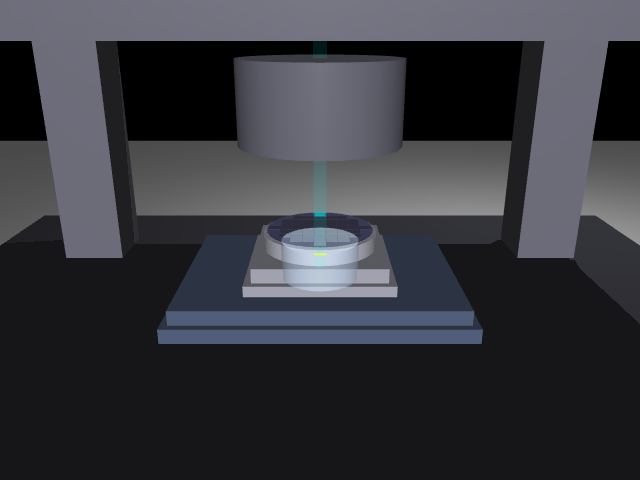
\includegraphics[width=0.8\textwidth]{scanning_3d.png}
    \caption{Captura de la simulación durante la fase de \textbf{SCAN}. Se observa el movimiento longitudinal sincronizado entre la retícula (superior) y la oblea (inferior).}
    \label{fig:scanning}
\end{figure}

\subsection{Fase 2: STEP}
Una vez que un die ha sido expuesto, la máquina entra en la fase de \textit{STEP}. En este estado, el escaneo se detiene y la cadena de la oblea realiza un movimiento lateral para posicionarse bajo el siguiente chip de la cuadrícula. 

La simulación modela la respuesta del \textit{Base Frame} (1400 kg) ante las fuerzas de reacción de los motores lineales, permitiendo analizar el tiempo de estabilización (\textit{settling time}) antes de iniciar el siguiente escaneo.

\end{document}
